% answers.tex —— 2011 年·四川卷·理科 · 参考答案与详细解析片段
% 由 tools/generate_projects.py 依来源总账自 2011/2011_数学真题_四川理_试题.md + 2011/2011_数学真题_四川理_解析正文.md + 2011/2011_数学真题_四川理_答案要点.md 生成，勿手改（改源 MD 后重跑）


\begin{gktip}
固定源 PDF 仅含题面、无答案页；以下解析与结论均由本库独立推导（非官方答案），并按 600 dpi 原页逐栏复核题面。原页未印分值，不补。

【源疑点】第 7 题四个选项均为函数图象，题干「$f(x)$ 的反函数的图象大致是」照录，选项图按原页拓扑重绘。第 15 题的圆柱在球内的两条母线与下底后半弧在原页画作虚线，照录。第 20 题设「$d$ 为非零实数」，当 $d=-1$ 时 $a_1=-1$，$a_2=a_3=\cdots=0$，此时 $\{a_n\}$ 不是等比数列，题面未排除该值，解析分 $d=-1$ 与 $d\neq-1$ 两类作答，题面照录不改。第 21 题第（2）问只排除 $P$ 与 $A$，$B$ 重合；当 $l\perp x$ 轴时 $AC\parallel BD$，点 $Q$ 不存在，解析按 $l$ 的斜率存在且不为 $0$ 处理，题面照录不改。
\end{gktip}

\begin{answer}
\gksolhead{1}{}

\textbf{题目}：

\Needspace{5\baselineskip}
有一容量为 $66$ 的样本，数据的分组及各组的频数如下：

\nopagebreak[4]
\[[11.5,15.5)\ \ 2 \qquad [15.5,19.5)\ \ 4 \qquad [19.5,23.5)\ \ 9 \qquad [23.5,27.5)\ \ 18\]
\nopagebreak[4]
\[[27.5,31.5)\ \ 11 \qquad [31.5,35.5)\ \ 12 \qquad [35.5,39.5)\ \ 7 \qquad [39.5,43.5)\ \ 3\]

根据样本的频率分布，估计数据落在 $[31.5,43.5)$ 的概率约是\mbox{（　　）}

（A）$\dfrac16$

（B）$\dfrac13$

（C）$\dfrac12$

（D）$\dfrac23$

\Needspace{4\baselineskip}
\textbf{解析}

\Needspace{5\baselineskip}
样本容量 $66$。落在 $[31.5,43.5)$ 内的分组为 $[31.5,35.5)$、$[35.5,39.5)$、$[39.5,43.5)$，频数分别为 $12$，$7$，$3$，合计
\nopagebreak[4]
\[12+7+3=22.\]
用频率估计概率，所求约为 $\dfrac{22}{66}=\dfrac13$。

逐项排除：$\dfrac16$ 对应频数 $66\times\dfrac16=11$，$\dfrac12$ 对应 $33$，$\dfrac23$ 对应 $44$，三者都不是 $22$；反过来，不在该区间内的频数为 $2+4+9+18+11=44$，恰为 $\dfrac23$，与 $\dfrac13$ 互补。

二次复算：八个分组的频数之和 $2+4+9+18+11+12+7+3=66$，与样本容量一致，故各频率之和为 $1$，所求频率就是 $1-\dfrac23=\dfrac13$。
故选 B。

\gkanswer{答案：B。}

\end{answer}
\begin{answer}
\gksolhead{2}{}

\textbf{题目}：

复数 $-\mathrm i+\dfrac{1}{\mathrm i}=$\mbox{（　　）}

（A）$-2\mathrm i$

（B）$\dfrac12\mathrm i$

（C）$0$

（D）$2\mathrm i$

\Needspace{4\baselineskip}
\textbf{解析}

\Needspace{5\baselineskip}
由 $(-\mathrm i)\cdot\mathrm i=-\mathrm i^2=1$ 知 $\dfrac1{\mathrm i}=-\mathrm i$，于是
\nopagebreak[4]
\[-\mathrm i+\frac1{\mathrm i}=-\mathrm i-\mathrm i=-2\mathrm i.\]

\Needspace{5\baselineskip}
逐项排除：把各选项与 $\mathrm i$ 相乘检验，看是否为 $1$。
\nopagebreak[4]
\[\frac{\mathrm i}{2}\cdot\mathrm i=\frac{\mathrm i^2}{2}=-\frac12,\qquad 0\cdot\mathrm i=0,\qquad 2\mathrm i\cdot\mathrm i=2\mathrm i^2=-2,\]
均不等于 $1$，故 $\dfrac{\mathrm i}{2}$，$0$，$2\mathrm i$ 都不等于 $\dfrac1{\mathrm i}$；而 $-\mathrm i$ 满足 $(-\mathrm i)\cdot\mathrm i=1$。

二次复算：$\mathrm i\cdot(-\mathrm i)=-\mathrm i^2=1$，故 $-\mathrm i$ 是 $\mathrm i$ 的倒数，即 $\dfrac1{\mathrm i}=-\mathrm i$；于是 $(-\mathrm i)+\dfrac1{\mathrm i}=-2\mathrm i$，与上面的结果一致。
故选 A。

\gkanswer{答案：A。}

\end{answer}
\begin{answer}
\gksolhead{3}{}

\textbf{题目}：

$l_1$，$l_2$，$l_3$ 是空间三条不同的直线，则下列命题正确的是\mbox{（　　）}

（A）$l_1\perp l_2$，$l_2\perp l_3\Rightarrow l_1\parallel l_3$

（B）$l_1\perp l_2$，$l_2\parallel l_3\Rightarrow l_1\perp l_3$

（C）$l_1\parallel l_2\parallel l_3\Rightarrow l_1$，$l_2$，$l_3$ 共面

（D）$l_1$，$l_2$，$l_3$ 共点 $\Rightarrow l_1$，$l_2$，$l_3$ 共面

\Needspace{4\baselineskip}
\textbf{解析}

记三条直线的方向向量为 $\boldsymbol a$，$\boldsymbol b$，$\boldsymbol c$，「$l_i\perp l_j$」即 $\boldsymbol a_i\cdot\boldsymbol a_j=0$，「$l_i\parallel l_j$」即两向量共线。

（B）若 $l_1\perp l_2$，$l_2\parallel l_3$，则存在 $\lambda\neq0$ 使 $\boldsymbol c=\lambda\boldsymbol b$，于是 $\boldsymbol a\cdot\boldsymbol c=\lambda(\boldsymbol a\cdot\boldsymbol b)=0$，即 $l_1\perp l_3$，正确。

（A）取 $l_1$，$l_2$，$l_3$ 分别为 $x$ 轴、$y$ 轴、$z$ 轴，两两垂直，但 $l_1\perp l_3$，不平行，错误。

（C）取过点 $(0,0,0)$，$(1,0,0)$，$(0,1,0)$ 且方向都是 $z$ 轴方向的三条平行直线，其中第三条不在前两条所在的平面 $y=0$ 内，三线不共面，错误。

（D）取过原点、方向分别为 $(1,0,0)$，$(0,1,0)$，$(1,1,1)$ 的三条直线，它们共点，但若共面则三方向向量共面，而 $\det\begin{pmatrix}1&0&0\\0&1&0\\1&1&1\end{pmatrix}=1\neq0$，不共面，错误。
故选 B。

\gkanswer{答案：B。}

\end{answer}
\begin{answer}
\gksolhead{4}{}

\textbf{题目}：

如图，正六边形 $ABCDEF$ 中，$\overrightarrow{BA}+\overrightarrow{CD}+\overrightarrow{EF}=$\mbox{（　　）}

（A）$\mathbf 0$

（B）$\overrightarrow{BE}$

（C）$\overrightarrow{AD}$

（D）$\overrightarrow{CF}$
\nopagebreak[4]
\begin{center}% 2011 年四川卷理科第 4 题：正六边形 ABCDEF，求 BA+CD+EF。
% 来源 PDF：普通高考/2011/2011四川理.pdf，SHA-256 116ce515679869425079ef4777505df3735ba4cba64847c9069b7d7acdb4fda4。
% 原页：第 1 页（A3 三栏）第 1 栏中部偏上，书页码 701。
% 重绘依据：照原页——上边 DE 水平、下边 BA 水平，D 在左上、E 在右上、C 在左、F 在右，
%   B 在左下、A 在右下；按正六边形作图，原页不画顶点圆点。
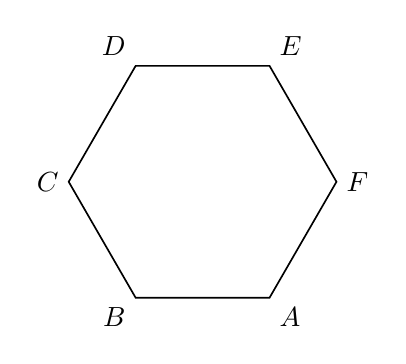
\begin{tikzpicture}[scale=1.7, >=stealth, semithick]
  \coordinate (A) at (0.5,-0.8660);
  \coordinate (B) at (-0.5,-0.8660);
  \coordinate (C) at (-1,0);
  \coordinate (D) at (-0.5,0.8660);
  \coordinate (E) at (0.5,0.8660);
  \coordinate (F) at (1,0);
  \draw (A) -- (B) -- (C) -- (D) -- (E) -- (F) -- cycle;
  \node at (A) [below right] {$A$};
  \node at (B) [below left] {$B$};
  \node at (C) [left] {$C$};
  \node at (D) [above left] {$D$};
  \node at (E) [above right] {$E$};
  \node at (F) [right] {$F$};
\end{tikzpicture}
\end{center}
\nopagebreak[4]
\Needspace{4\baselineskip}
\textbf{解析}

\Needspace{5\baselineskip}
以正六边形中心为原点、边长为 $1$ 建系，按原图 $A$ 在右下、$B$ 在左下、$C$ 在左、$D$ 在左上、$E$ 在右上、$F$ 在右：
\nopagebreak[4]
\[A\left(\tfrac12,-\tfrac{\sqrt3}{2}\right),\ B\left(-\tfrac12,-\tfrac{\sqrt3}{2}\right),\ C(-1,0),\ D\left(-\tfrac12,\tfrac{\sqrt3}{2}\right),\ E\left(\tfrac12,\tfrac{\sqrt3}{2}\right),\ F(1,0).\]
\Needspace{5\baselineskip}
于是
\nopagebreak[4]
\[\overrightarrow{BA}=(1,0),\quad \overrightarrow{CD}=\left(\tfrac12,\tfrac{\sqrt3}{2}\right),\quad \overrightarrow{EF}=\left(\tfrac12,-\tfrac{\sqrt3}{2}\right),\]
\nopagebreak[4]
\[\overrightarrow{BA}+\overrightarrow{CD}+\overrightarrow{EF}=(2,0).\]
而 $\overrightarrow{CF}=F-C=(2,0)$，恰与之相等。

逐项排除：$\mathbf 0$ 显然不符；$\overrightarrow{BE}=\left(1,\sqrt3\right)$，$\overrightarrow{AD}=\left(-1,\sqrt3\right)$，均不等于 $(2,0)$。

几何验证：正六边形中 $\overrightarrow{CD}=\overrightarrow{AF}$，故 $\overrightarrow{BA}+\overrightarrow{CD}=\overrightarrow{BA}+\overrightarrow{AF}=\overrightarrow{BF}$，再由 $\overrightarrow{BF}+\overrightarrow{EF}=\overrightarrow{CF}$ 亦得 $\overrightarrow{CF}$，两条路子一致。
故选 D。

\gkanswer{答案：D。}

\end{answer}
\begin{answer}
\gksolhead{5}{}

\textbf{题目}：

“函数 $f(x)$ 在点 $x=x_0$ 处有定义”是“$f(x)$ 在点 $x=x_0$ 处连续”的\mbox{（　　）}

（A）充分而不必要的条件

（B）必要而不充分的条件

（C）充要条件

（D）既不充分也不必要的条件

\Needspace{4\baselineskip}
\textbf{解析}

设 $p$：$f(x)$ 在 $x=x_0$ 处有定义；$q$：$f(x)$ 在 $x=x_0$ 处连续。

连续性要求函数在该点有定义，且 $\lim\limits_{x\to x_0}f(x)=f(x_0)$，故 $q\Rightarrow p$，必要性成立。

\Needspace{5\baselineskip}
反之，取
\nopagebreak[4]
\[f(x)=\begin{cases}\dfrac1x,&x\neq0,\\[2pt] 0,&x=0,\end{cases}\]
则 $f$ 在 $x=0$ 处有定义，但 $x\to0$ 时 $f(x)$ 无极限，故在 $x=0$ 处不连续，$p\not\Rightarrow q$，充分性不成立。

故 $p$ 是 $q$ 的必要而不充分条件。逐项核对：A 把充分、必要颠倒，C 误判为等价，D 忽视了「连续必有定义」。
故选 B。

\gkanswer{答案：B。}

\end{answer}
\begin{answer}
\gksolhead{6}{}

\textbf{题目}：

在 $\triangle ABC$ 中，$\sin^2A\leqslant\sin^2B+\sin^2C-\sin B\sin C$，则 $A$ 的取值范围是\mbox{（　　）}

（A）$\left(0,\dfrac{\pi}{6}\right]$

（B）$\left[\dfrac{\pi}{6},\pi\right)$

（C）$\left(0,\dfrac{\pi}{3}\right]$

（D）$\left[\dfrac{\pi}{3},\pi\right)$

\Needspace{4\baselineskip}
\textbf{解析}

\Needspace{5\baselineskip}
由正弦定理 $\dfrac{a}{\sin A}=\dfrac{b}{\sin B}=\dfrac{c}{\sin C}=2R$，条件 $\sin^2A\leqslant\sin^2B+\sin^2C-\sin B\sin C$ 两边同乘 $(2R)^2$ 得
\nopagebreak[4]
\[a^2\leqslant b^2+c^2-bc.\]
\Needspace{5\baselineskip}
又由余弦定理 $a^2=b^2+c^2-2bc\cos A$，两式相减：
\nopagebreak[4]
\[b^2+c^2-2bc\cos A\leqslant b^2+c^2-bc\iff -2bc\cos A\leqslant-bc\iff\cos A\geqslant\frac12.\]
因 $A\in(0,\pi)$，故 $A\in\left(0,\dfrac{\pi}{3}\right]$。

端点核对：$A=\dfrac{\pi}{3}$ 时 $\cos A=\dfrac12$，条件取等号，成立；$A\to0^+$ 时条件严格成立，但三角形内角 $A>0$，故左端不取 $0$。若 $A\geqslant\dfrac{\pi}{3}$ 而 $A\neq\dfrac{\pi}{3}$，则 $\cos A<\dfrac12$，条件反向不成立。

逐项排除：A 的 $\dfrac{\pi}{6}$ 过强，B、D 把区间写反或含 $\dfrac{\pi}{3}$ 以外的值。
故选 C。

\gkanswer{答案：C。}

\end{answer}
\begin{answer}
\gksolhead{7}{}

\textbf{题目}：

已知 $f(x)$ 是 $\mathbf R$ 上的奇函数，且当 $x>0$ 时，$f(x)=\left(\dfrac12\right)^x+1$，则 $f(x)$ 的反函数的图象大致是\mbox{（　　）}

（A）图 A

（B）图 B

（C）图 C

（D）图 D
\nopagebreak[4]
\begin{center}% 2011 年四川卷理科第 7 题：四个选项的函数图象（选项图）。
% 来源 PDF：普通高考/2011/2011四川理.pdf，SHA-256 116ce515679869425079ef4777505df3735ba4cba64847c9069b7d7acdb4fda4。
% 原页：第 1 页（A3 三栏）第 1 栏下部接第 2 栏上部，书页码 701。
% 重绘依据：题设 f 为 R 上奇函数，x>0 时 f(x)=(1/2)^x+1，故 f(0)=0，
%   x<0 时 f(x)=-(2^x+1)；f 在 R 上单射，反函数 g=f^{-1} 满足
%   x∈(1,2) 时 g(x)=log_{1/2}(x-1)，x∈(-2,-1) 时 g(x)=log_2(-x-1)，g(0)=0。
%   照原页：(A) 为 y=g(x)；(B) 为 y=f(x)；(C) 为 y=f(-x)；(D) 为 y=-g(x)。
%   端点空心圆、原点实心点、竖直渐近线位置均照原页，不按比例。
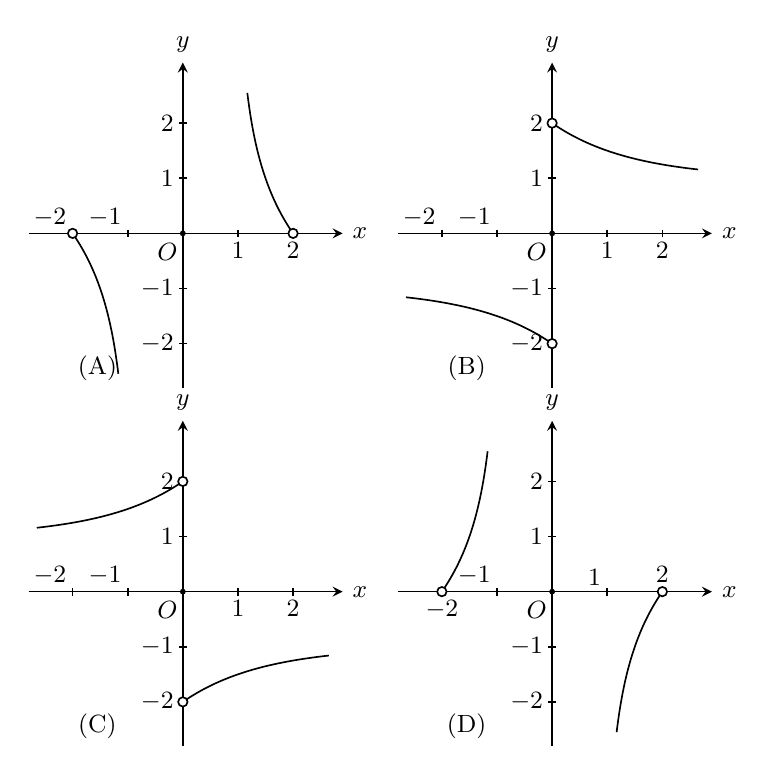
\begin{tikzpicture}[scale=0.70, >=stealth, semithick, font=\small,
  dec/.style={fill=white, draw=black}]

  % ================= (A) y = f^{-1}(x) =================
  \begin{scope}
    \draw[->] (-2.8,0) -- (2.9,0) node[right] {$x$};
    \draw[->] (0,-2.8) -- (0,3.1) node[above] {$y$};
    \foreach \t in {-2,-1,1,2} { \draw (\t,0.07) -- (\t,-0.07); }
    \foreach \t in {-2,-1,1,2} { \draw (0.07,\t) -- (-0.07,\t); }
    \node[above left, inner sep=2pt] at (-2,0) {$-2$};
    \node[above left, inner sep=2pt] at (-1,0) {$-1$};
    \node[below, inner sep=3pt] at (1,0) {$1$};
    \node[below, inner sep=3pt] at (2,0) {$2$};
    \node[left, inner sep=3pt] at (0,1) {$1$};
    \node[left, inner sep=3pt] at (0,2) {$2$};
    \node[left, inner sep=3pt] at (0,-1) {$-1$};
    \node[left, inner sep=3pt] at (0,-2) {$-2$};
    \node at (-0.28,-0.34) {$O$};
    \draw[domain=-1.96:-1.17, samples=70] plot (\x,{ln(-\x-1)/ln(2)});
    \draw[domain=1.17:1.96, samples=70] plot (\x,{-ln(\x-1)/ln(2)});
    \node[dec] at (-2,0) [circle, inner sep=0pt, minimum size=3.4pt] {};
    \node[dec] at (2,0)  [circle, inner sep=0pt, minimum size=3.4pt] {};
    \fill (0,0) circle (1.5pt);
    \node at (-1.55,-2.45) {(A)};
  \end{scope}

  % ================= (B) y = f(x) =================
  \begin{scope}[xshift=6.7cm]
    \draw[->] (-2.8,0) -- (2.9,0) node[right] {$x$};
    \draw[->] (0,-2.8) -- (0,3.1) node[above] {$y$};
    \foreach \t in {-2,-1,1,2} { \draw (\t,0.07) -- (\t,-0.07); }
    \foreach \t in {-2,-1,1,2} { \draw (0.07,\t) -- (-0.07,\t); }
    \node[above left, inner sep=2pt] at (-2,0) {$-2$};
    \node[above left, inner sep=2pt] at (-1,0) {$-1$};
    \node[below, inner sep=3pt] at (1,0) {$1$};
    \node[below, inner sep=3pt] at (2,0) {$2$};
    \node[left, inner sep=3pt] at (0,1) {$1$};
    \node[left, inner sep=3pt] at (0,2) {$2$};
    \node[left, inner sep=3pt] at (0,-1) {$-1$};
    \node[left, inner sep=3pt] at (0,-2) {$-2$};
    \node at (-0.28,-0.34) {$O$};
    \draw[domain=0.06:2.65, samples=70] plot (\x,{exp(-\x*ln(2))+1});
    \draw[domain=-2.65:-0.06, samples=70] plot (\x,{-exp(\x*ln(2))-1});
    \node[dec] at (0,2) [circle, inner sep=0pt, minimum size=3.4pt] {};
    \node[dec] at (0,-2) [circle, inner sep=0pt, minimum size=3.4pt] {};
    \fill (0,0) circle (1.5pt);
    \node at (-1.55,-2.45) {(B)};
  \end{scope}

  % ================= (C) y = f(-x) =================
  \begin{scope}[yshift=-6.5cm]
    \draw[->] (-2.8,0) -- (2.9,0) node[right] {$x$};
    \draw[->] (0,-2.8) -- (0,3.1) node[above] {$y$};
    \foreach \t in {-2,-1,1,2} { \draw (\t,0.07) -- (\t,-0.07); }
    \foreach \t in {-2,-1,1,2} { \draw (0.07,\t) -- (-0.07,\t); }
    \node[above left, inner sep=2pt] at (-2,0) {$-2$};
    \node[above left, inner sep=2pt] at (-1,0) {$-1$};
    \node[below, inner sep=3pt] at (1,0) {$1$};
    \node[below, inner sep=3pt] at (2,0) {$2$};
    \node[left, inner sep=3pt] at (0,1) {$1$};
    \node[left, inner sep=3pt] at (0,2) {$2$};
    \node[left, inner sep=3pt] at (0,-1) {$-1$};
    \node[left, inner sep=3pt] at (0,-2) {$-2$};
    \node at (-0.28,-0.34) {$O$};
    \draw[domain=-2.65:-0.06, samples=70] plot (\x,{exp(\x*ln(2))+1});
    \draw[domain=0.06:2.65, samples=70] plot (\x,{-exp(-\x*ln(2))-1});
    \node[dec] at (0,2) [circle, inner sep=0pt, minimum size=3.4pt] {};
    \node[dec] at (0,-2) [circle, inner sep=0pt, minimum size=3.4pt] {};
    \fill (0,0) circle (1.5pt);
    \node at (-1.55,-2.45) {(C)};
  \end{scope}

  % ================= (D) y = -f^{-1}(x) =================
  \begin{scope}[xshift=6.7cm, yshift=-6.5cm]
    \draw[->] (-2.8,0) -- (2.9,0) node[right] {$x$};
    \draw[->] (0,-2.8) -- (0,3.1) node[above] {$y$};
    \foreach \t in {-2,-1,1,2} { \draw (\t,0.07) -- (\t,-0.07); }
    \foreach \t in {-2,-1,1,2} { \draw (0.07,\t) -- (-0.07,\t); }
    \node[below, inner sep=3pt] at (-2,0) {$-2$};
    \node[above left, inner sep=2pt] at (-1,0) {$-1$};
    \node[above left, inner sep=2pt] at (1,0) {$1$};
    \node[above, inner sep=3pt] at (2,0) {$2$};
    \node[left, inner sep=3pt] at (0,1) {$1$};
    \node[left, inner sep=3pt] at (0,2) {$2$};
    \node[left, inner sep=3pt] at (0,-1) {$-1$};
    \node[left, inner sep=3pt] at (0,-2) {$-2$};
    \node at (-0.28,-0.34) {$O$};
    \draw[domain=-1.96:-1.17, samples=70] plot (\x,{-ln(-\x-1)/ln(2)});
    \draw[domain=1.17:1.96, samples=70] plot (\x,{ln(\x-1)/ln(2)});
    \node[dec] at (-2,0) [circle, inner sep=0pt, minimum size=3.4pt] {};
    \node[dec] at (2,0)  [circle, inner sep=0pt, minimum size=3.4pt] {};
    \fill (0,0) circle (1.5pt);
    \node at (-1.55,-2.45) {(D)};
  \end{scope}

\end{tikzpicture}
\end{center}
\nopagebreak[4]
\Needspace{4\baselineskip}
\textbf{解析}

\Needspace{5\baselineskip}
先补出 $x\leqslant0$ 的表达式。$f$ 是 $\mathbf R$ 上的奇函数，故 $f(0)=0$；当 $x<0$ 时 $-x>0$，
\nopagebreak[4]
\[f(x)=-f(-x)=-\left[\left(\frac12\right)^{-x}+1\right]=-(2^x+1).\]

分段看值域与单调性：$x>0$ 时 $f(x)=\left(\dfrac12\right)^x+1\in(1,2)$ 且递减；$x<0$ 时 $f(x)=-(2^x+1)\in(-2,-1)$ 且递减。三段值域 $(-2,-1)$，$\{0\}$，$(1,2)$ 互不相交，故 $f$ 是单射，反函数 $g=f^{-1}$ 存在。

求 $g$ 的两支：
\begin{itemize}
\item $y\in(1,2)$ 时，由 $y=\left(\dfrac12\right)^x+1$ 得 $\left(\dfrac12\right)^x=y-1$，$x=\log_{\frac12}(y-1)$，即 $g(x)=\log_{\frac12}(x-1)$，定义域 $(1,2)$，递减，$x\to1^+$ 时 $g\to+\infty$，$x\to2^-$ 时 $g\to0^+$；
\item $y\in(-2,-1)$ 时，由 $y=-(2^x+1)$ 得 $2^x=-y-1$，$x=\log_2(-y-1)$，即 $g(x)=\log_2(-x-1)$，定义域 $(-2,-1)$，递减，$x\to-2^+$ 时 $g\to0^-$，$x\to-1^-$ 时 $g\to-\infty$；
\item $g(0)=0$。
\end{itemize}

于是 $y=g(x)$ 的图象：左支在 $x\in(-2,-1)$ 上为负值、随 $x$ 增大降到 $-\infty$，渐近线 $x=-1$；右支在 $x\in(1,2)$ 上为正值、自 $+\infty$ 降到 $0$，渐近线 $x=1$；再过一个实心点 $(0,0)$。

对照四个选项：(A) 左支由 $(-2,0)$ 的空心点下降、渐近线 $x=-1$，右支自 $x=1$ 附近的高处下降、止于 $(2,0)$ 的空心点，过原点，与此完全一致；(B) 是 $y=f(x)$ 本身（$x>0$ 支从 $(0,2)$ 递减，$x<0$ 支趋于 $(0,-2)$）；(C) 是 $y=f(-x)$（两支单调递增）；(D) 是 $y=-g(x)$（左支上升而右支上升，增减方向与 $g$ 相反）。故只有 (A) 正确。

二次复算：取 $x=\dfrac32$，$g\left(\dfrac32\right)=\log_{\frac12}\dfrac12=1$，即 $(1.5,1)$ 在图上，而 $f(1)=\dfrac12+1=\dfrac32$，互为反函数，自洽；(A) 中该点位于右支中部。
故选 A。

\gkanswer{答案：A。}

\end{answer}
\begin{answer}
\gksolhead{8}{}

\textbf{题目}：

数列 $\{a_n\}$ 的首项为 $3$，$\{b_n\}$ 为等差数列且 $b_n=a_{n+1}-a_n$（$n\in\mathbf N^*$）。若 $b_3=-2$，$b_{10}=12$，则 $a_8=$\mbox{（　　）}

（A）$0$

（B）$3$

（C）$8$

（D）$11$

\Needspace{4\baselineskip}
\textbf{解析}

\Needspace{5\baselineskip}
$\{b_n\}$ 为等差数列，公差
\nopagebreak[4]
\[d_b=\frac{b_{10}-b_3}{10-3}=\frac{12-(-2)}{7}=2,\]
故 $b_n=b_3+2(n-3)=2n-8$，特别地 $b_1=-6$，$b_7=6$。

\Needspace{5\baselineskip}
由 $b_n=a_{n+1}-a_n$ 累加（$n=1,2,\cdots,7$）得
\nopagebreak[4]
\[a_8-a_1=\sum_{k=1}^{7}b_k=\frac{7(b_1+b_7)}{2}=\frac{7(-6+6)}{2}=0,\]
故 $a_8=a_1=3$。

二次复算（逐项递推）：$b_1=-6$，$b_2=-4$，$b_3=-2$，$b_4=0$，$b_5=2$，$b_6=4$，$b_7=6$，于是 $a_2=-3$，$a_3=-7$，$a_4=-9$，$a_5=-9$，$a_6=-7$，$a_7=-3$，$a_8=3$，与上式一致；并核 $b_3=a_4-a_3=-9-(-7)=-2$，与题设相符。
故选 B。

\gkanswer{答案：B。}

\end{answer}
\begin{answer}
\gksolhead{9}{}

\textbf{题目}：

某运输公司有 $12$ 名驾驶员和 $19$ 名工人，有 $8$ 辆载重量为 $10$ 吨的甲型卡车和 $7$ 辆载重量为 $6$ 吨的乙型卡车。某天需运往 $A$ 地至少 $72$ 吨的货物，派用的每辆车需载满且只运送一次，派用的每辆甲型卡车需配 $2$ 名工人，运送一次可得利润 $450$ 元；派用的每辆乙型卡车需配 $1$ 名工人，运送一次可得利润 $350$ 元，该公司合理计划当天派用甲、乙卡车的车辆数，可得最大利润 $z=$\mbox{（　　）}

（A）$4650$ 元

（B）$4700$ 元

（C）$4900$ 元

（D）$5000$ 元

\Needspace{4\baselineskip}
\textbf{解析}

设派用甲型卡车 $x$ 辆、乙型卡车 $y$ 辆（$x$，$y$ 为非负整数），则

\begin{itemize}
\item 车辆数：$x\leqslant8$，$y\leqslant7$；
\item 驾驶员：每车一名，$x+y\leqslant12$；
\item 工人：$2x+y\leqslant19$；
\item 运量：每车满载且各运一次，$10x+6y\geqslant72$；
\item 目标：$z=450x+350y$。
\end{itemize}

由 $x\leqslant8$，$y\leqslant7$，$x+y\leqslant12$ 及 $2x+y\leqslant19$ 得可行域的整数点，逐个代入 $z$ 比较：

\begin{center}
\begin{tabular}{lll}
\toprule
$(x,y)$ & 运量 $10x+6y$ & 利润 $z$ \\
\midrule
$(8,3)$ & $98$ & $4650$ \\
$(7,5)$ & $100$ & $4900$ \\
$(6,6)$ & $96$ & $4800$ \\
$(5,7)$ & $92$ & $4700$ \\
$(7,4)$ & $94$ & $4550$ \\
\bottomrule
\end{tabular}
\end{center}

其中 $(8,3)$ 受 $2x+y\leqslant19$ 限制（$19$ 恰满），$(7,5)$ 受 $2x+y=19$ 限制且 $x+y=12$ 恰满，$(6,6)$，$(5,7)$ 受 $x+y\leqslant12$ 限制。最大值在 $(7,5)$ 取得，$z=450\times7+350\times5=3150+1750=4900$。

验证边界：若忽略驾驶员约束而取 $(6,7)$，得 $2700+2450=5150>4900$，但 $6+7=13>12$，没有足够驾驶员，不可行；这正说明 $x+y\leqslant12$ 必须计入。
故选 C。

\gkanswer{答案：C。}

\end{answer}
\begin{answer}
\gksolhead{10}{}

\textbf{题目}：

在抛物线 $y=x^2+ax-5$（$a\neq0$）上取横坐标为 $x_1=-4$，$x_2=2$ 的两点，经过两点引一条割线，有平行于该割线的一条直线同时与抛物线和圆 $5x^2+5y^2=36$ 相切，则抛物线顶点的坐标为\mbox{（　　）}

（A）$(-2,-9)$

（B）$(0,-5)$

（C）$(2,-9)$

（D）$(1,-6)$

\Needspace{4\baselineskip}
\textbf{解析}

\Needspace{5\baselineskip}
抛物线 $y=x^2+ax-5$ 上横坐标为 $-4$，$2$ 的两点为
\nopagebreak[4]
\[(-4,\,11-4a),\qquad (2,\,2a-1),\]
\Needspace{5\baselineskip}
割线斜率
\nopagebreak[4]
\[k=\frac{(2a-1)-(11-4a)}{2-(-4)}=\frac{6a-12}{6}=a-2.\]
（这也等于抛物线在 $x=\dfrac{-4+2}{2}=-1$ 处的导数 $2(-1)+a=a-2$。）

\Needspace{5\baselineskip}
设与该割线平行的切线为 $y=(a-2)x+b$。与抛物线联立：
\nopagebreak[4]
\[x^2+ax-5=(a-2)x+b\iff x^2+2x-(5+b)=0,\]
相切要求判别式为 $0$：$4+4(5+b)=0$，得 $b=-6$。故切线为 $(a-2)x-y-6=0$。

\Needspace{5\baselineskip}
圆 $5x^2+5y^2=36$ 即 $x^2+y^2=\dfrac{36}{5}$，半径 $r=\dfrac{6}{\sqrt5}$。切线与之相切，圆心到直线距离等于半径：
\nopagebreak[4]
\[\frac{6}{\sqrt{(a-2)^2+1}}=\frac{6}{\sqrt5}\iff (a-2)^2+1=5\iff (a-2)^2=4,\]
故 $a=4$ 或 $a=0$；题设 $a\neq0$，取 $a=4$。

顶点坐标：$x=-\dfrac a2=-2$，$y=-\dfrac{a^2}{4}-5=-4-5=-9$，即 $(-2,-9)$。

二次复算：$a=4$ 时抛物线 $y=x^2+4x-5$，割线斜率 $2$，与它平行且与抛物线相切的直线为 $y=2x-6$（$x^2+4x-5=2x-6$ 即 $(x+1)^2=0$），原点到 $2x-y-6=0$ 的距离为 $\dfrac{6}{\sqrt5}=r$，确与圆相切。
故选 A。

\gkanswer{答案：A。}

\end{answer}
\begin{answer}
\gksolhead{11}{}

\textbf{题目}：

已知定义在 $[0,+\infty)$ 上的函数 $f(x)$ 满足 $f(x)=3f(x+2)$，当 $x\in[0,2)$ 时，$f(x)=-x^2+2x$。设 $f(x)$ 在 $[2n-2,2n)$ 上的最大值为 $a_n$（$n\in\mathbf N^*$），且 $\{a_n\}$ 的前 $n$ 项和为 $S_n$，则 $\lim\limits_{n\to\infty}S_n=$\mbox{（　　）}

（A）$3$

（B）$\dfrac52$

（C）$2$

（D）$\dfrac32$

\Needspace{4\baselineskip}
\textbf{解析}

由 $f(x)=3f(x+2)$ 得 $f(x+2)=\dfrac13f(x)$，即每向右平移 $2$ 个单位，函数值变为原来的 $\dfrac13$。

\Needspace{5\baselineskip}
任取 $x\in[2n-2,2n)$，令 $u=x-(2n-2)\in[0,2)$，反复用递推式 $n-1$ 次得
\nopagebreak[4]
\[f(x)=f\bigl(u+2(n-1)\bigr)=\frac{1}{3^{n-1}}f(u).\]
\Needspace{5\baselineskip}
而 $u\in[0,2)$ 时 $f(u)=-u^2+2u=-(u-1)^2+1$，在 $u=1$ 处取最大值 $1$（$u=1\in[0,2)$），最小趋近于 $0$。故
\nopagebreak[4]
\[a_n=\frac{1}{3^{n-1}}\cdot1=\left(\frac13\right)^{n-1}.\]
\Needspace{5\baselineskip}
于是 $\{a_n\}$ 是首项 $1$、公比 $\dfrac13$ 的等比数列，
\nopagebreak[4]
\[S_n=\frac{1-\left(\frac13\right)^n}{1-\frac13}=\frac32\left[1-\left(\frac13\right)^n\right]\xrightarrow[n\to\infty]{}\frac32.\]

二次复算：$a_1=1$，$a_2=\dfrac13$，$a_3=\dfrac19$，直接由 $f$ 在 $[2,4)$ 上的最大值检验：$x\in[2,4)$ 时 $f(x)=\dfrac13f(x-2)$，$x-2\in[0,2)$，最大值 $\dfrac13$，相符。
故选 D。

\gkanswer{答案：D。}

\end{answer}
\begin{answer}
\gksolhead{12}{}

\textbf{题目}：

在集合 $\{1,2,3,4,5\}$ 中任取一个偶数 $a$ 和一个奇数 $b$ 构成以原点为起点的向量 $\boldsymbol\alpha=(a,b)$。从所有得到的以原点为起点的向量中任取两个向量为邻边作平行四边形。记所有作成的平行四边形的个数为 $n$，其中面积不超过 $4$ 的平行四边形的个数为 $m$，则 $\dfrac{m}{n}=$\mbox{（　　）}

（A）$\dfrac{4}{15}$

（B）$\dfrac13$

（C）$\dfrac25$

（D）$\dfrac23$

\Needspace{4\baselineskip}
\textbf{解析}

\Needspace{5\baselineskip}
偶数 $a\in\{2,4\}$ 有 $2$ 种取法，奇数 $b\in\{1,3,5\}$ 有 $3$ 种取法，共得 $6$ 个向量：
\nopagebreak[4]
\[(2,1),\ (2,3),\ (2,5),\ (4,1),\ (4,3),\ (4,5).\]
\Needspace{5\baselineskip}
任两个都不共线（否则对应分量成比例，逐一检查无此情形），故任取两个都作成平行四边形，个数
\nopagebreak[4]
\[n=\mathrm C_6^2=15.\]
以 $\boldsymbol\alpha=(a_1,b_1)$，$\boldsymbol\beta=(a_2,b_2)$ 为邻边的平行四边形面积为 $S=|a_1b_2-a_2b_1|$。逐个基本事件计算：

\begin{center}
\begin{tabular}{llllll}
\toprule
向量对 & $S$ & 向量对 & $S$ & 向量对 & $S$ \\
\midrule
$(2,1),(2,3)$ & $4$ & $(2,1),(2,5)$ & $8$ & $(2,1),(4,1)$ & $2$ \\
$(2,1),(4,3)$ & $2$ & $(2,1),(4,5)$ & $6$ & $(2,3),(2,5)$ & $4$ \\
$(2,3),(4,1)$ & $10$ & $(2,3),(4,3)$ & $6$ & $(2,3),(4,5)$ & $2$ \\
$(2,5),(4,1)$ & $18$ & $(2,5),(4,3)$ & $14$ & $(2,5),(4,5)$ & $10$ \\
$(4,1),(4,3)$ & $8$ & $(4,1),(4,5)$ & $16$ & $(4,3),(4,5)$ & $8$ \\
\bottomrule
\end{tabular}
\end{center}

\Needspace{5\baselineskip}
$S\leqslant4$ 的为 $4$，$2$，$2$，$4$，$2$ 共 $5$ 个，故 $m=5$，
\nopagebreak[4]
\[\frac mn=\frac{5}{15}=\frac13.\]

二次复算：按 $a$ 的取值分组核面积和——两个向量都取自 $a=2$ 的 $3$ 对，面积和为 $4+8+4=16$；都取自 $a=4$ 的 $3$ 对，和为 $8+16+8=32$；跨组的 $9$ 对，和为 $2+2+6+10+6+2+18+14+10=70$。三部分合计 $16+32+70=118$，与上表逐对相加所得相同，说明表内 $15$ 对无重无漏。
故选 B。

\gkanswer{答案：B。}

\end{answer}
\begin{answer}
\gksolhead{13}{}

\textbf{题目}：

计算 $\left(\lg\dfrac14-\lg 25\right)\div 100^{-\frac12}=$ $\underline{\qquad}$。

\Needspace{4\baselineskip}
\textbf{解析}

\Needspace{5\baselineskip}
先算括号：
\nopagebreak[4]
\[\lg\frac14=-\lg4,\qquad \lg\frac14-\lg25=-(\lg4+\lg25)=-\lg100=-2.\]
\Needspace{5\baselineskip}
再算指数：$100^{-\frac12}=\dfrac{1}{\sqrt{100}}=\dfrac1{10}$。故
\nopagebreak[4]
\[\left(\lg\frac14-\lg25\right)\div100^{-\frac12}=(-2)\div\frac1{10}=-20.\]

二次复算：$-2\times10=-20$；也可写成 $\lg\dfrac{1}{4\times25}=\lg\dfrac1{100}=-2$，同一结果。

\gkanswer{答案：$-20$。}

\end{answer}
\begin{answer}
\gksolhead{14}{}

\textbf{题目}：

双曲线 $\dfrac{x^2}{64}-\dfrac{y^2}{36}=1$ 上一点 $P$ 到双曲线右焦点的距离是 $4$，那么点 $P$ 到左准线的距离是 $\underline{\qquad}$。

\Needspace{4\baselineskip}
\textbf{解析}

双曲线 $\dfrac{x^2}{64}-\dfrac{y^2}{36}=1$ 中 $a=8$，$b=6$，$c=\sqrt{64+36}=10$，离心率 $e=\dfrac ca=\dfrac54$，左准线为 $x=-\dfrac{a^2}{c}=-\dfrac{32}{5}$，右准线为 $x=\dfrac{32}{5}$。

\Needspace{5\baselineskip}
设 $F_1$，$F_2$ 为左、右焦点，则 $|PF_2|=4$。左支上的点到右焦点的距离至少为 $c+a=18$，故 $4<18$ 说明 $P$ 在右支上（右支上到右焦点的距离最小为 $c-a=2$，$4\geqslant2$ 亦可取到）。由双曲线定义
\nopagebreak[4]
\[|PF_1|-|PF_2|=2a=16\implies|PF_1|=20.\]
\Needspace{5\baselineskip}
再由第二定义，$P$ 到左准线的距离
\nopagebreak[4]
\[d=\frac{|PF_1|}{e}=20\times\frac45=16.\]

代回验证：右支上点满足 $|PF_2|=e\left(x_P-\dfrac{32}{5}\right)$，故 $x_P-\dfrac{32}{5}=\dfrac{4}{5/4}=\dfrac{16}{5}$，$x_P=\dfrac{48}{5}$，于是 $d=x_P+\dfrac{32}{5}=\dfrac{48+32}{5}=16$，与上式一致。

\gkanswer{答案：$16$。}

\end{answer}
\begin{answer}
\gksolhead{15}{}

\textbf{题目}：

如图，半径为 $R$ 的球 $O$ 中有一内接圆柱。当圆柱的侧面积最大时，球的表面积与该圆柱的侧面积之差是 $\underline{\qquad}$。
\nopagebreak[4]
\begin{center}% 2011 年四川卷理科第 15 题：半径为 R 的球 O 的内接圆柱（侧面积最大时）。
% 来源 PDF：普通高考/2011/2011四川理.pdf，SHA-256 116ce515679869425079ef4777505df3735ba4cba64847c9069b7d7acdb4fda4。
% 原页：第 1 页（A3 三栏）第 2 栏下部，书页码 701。
% 重绘依据：照原页——外轮廓为球的大圆；圆柱上下底画成扁椭圆，
%   上底整圈实线（俯视可见），下底前半实线、后半虚线；圆柱两条母线为虚线；
%   球的赤道前半实线、后半虚线；O 为球心（实心点），R 由 O 连到上底圆周上一点（虚线）。
% 比例取 r=0.73R、高=0.68R（r^2+(h/2)^2=R^2），与原页大致相符，不严格按比例。
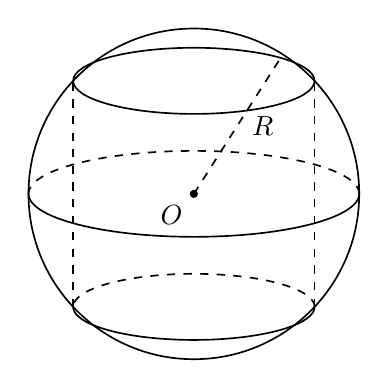
\begin{tikzpicture}[scale=1.05, >=stealth, semithick]
  % 球的大圆
  \draw (0,0) circle (2);

  % 球的赤道：前半实线，后半虚线
  \draw[domain=180:360, samples=60] plot ({2*cos(\x)},{0.52*sin(\x)});
  \draw[dashed, domain=0:180, samples=60] plot ({2*cos(\x)},{0.52*sin(\x)});

  % 圆柱上底（整圈可见）
  \draw (0,1.367) ellipse ({1.46} and {0.40});

  % 圆柱下底：前半实线，后半虚线
  \draw[domain=180:360, samples=60] plot ({1.46*cos(\x)},{-1.367+0.40*sin(\x)});
  \draw[dashed, domain=0:180, samples=60] plot ({1.46*cos(\x)},{-1.367+0.40*sin(\x)});

  % 圆柱母线（原页为虚线）
  \draw[dashed] (-1.46,-1.367) -- (-1.46,1.367);
  \draw[dashed] (1.46,-1.367) -- (1.46,1.367);

  % 球心与半径
  \fill (0,0) circle (1.4pt);
  \node[below left, inner sep=2pt] at (-0.06,-0.06) {$O$};
  \draw[dashed] (0,0) -- (1.05,1.645);
  \node[below right, inner sep=1pt] at (0.66,0.98) {$R$};
\end{tikzpicture}
\end{center}
\nopagebreak[4]
\Needspace{4\baselineskip}
\textbf{解析}

\Needspace{5\baselineskip}
设内接圆柱底面半径为 $r$、高为 $h$。圆柱两底圆心与球心共线，底面圆在球内，故
\nopagebreak[4]
\[r^2+\left(\frac h2\right)^2=R^2.\]
\Needspace{5\baselineskip}
侧面积
\nopagebreak[4]
\[S=2\pi rh=2\pi r\cdot2\sqrt{R^2-r^2}=4\pi r\sqrt{R^2-r^2}.\]
\Needspace{5\baselineskip}
由 $r^2(R^2-r^2)\leqslant\left(\dfrac{r^2+R^2-r^2}{2}\right)^2=\dfrac{R^4}{4}$，等号当 $r^2=R^2-r^2$ 即 $r=\dfrac{R}{\sqrt2}$ 时成立，此时
\nopagebreak[4]
\[S_{\max}=4\pi\sqrt{\frac{R^4}{4}}=2\pi R^2,\qquad h=2\sqrt{R^2-\frac{R^2}{2}}=\sqrt2R.\]
\Needspace{5\baselineskip}
球表面积 $4\pi R^2$，故所求之差为
\nopagebreak[4]
\[4\pi R^2-2\pi R^2=2\pi R^2.\]

二次复算：$S^2=16\pi^2r^2(R^2-r^2)$，记 $t=r^2$，则 $t(R^2-t)$ 在 $t=\dfrac{R^2}{2}$ 取最大值 $\dfrac{R^4}{4}$，$S_{\max}=4\pi\cdot\dfrac{R^2}{2}=2\pi R^2$，一致。

\gkanswer{答案：$2\pi R^2$。}

\end{answer}
\begin{answer}
\gksolhead{16}{}

\textbf{题目}：

函数 $f(x)$ 的定义域为 $A$，若 $x_1$，$x_2\in A$ 且 $f(x_1)=f(x_2)$ 时总有 $x_1=x_2$，则称 $f(x)$ 为单函数。例如，函数 $f(x)=2x+1$（$x\in\mathbf R$）是单函数。下列命题：

① 函数 $f(x)=x^2$（$x\in\mathbf R$）是单函数；

② 若 $f(x)$ 为单函数，$x_1$，$x_2\in A$ 且 $x_1\neq x_2$，则 $f(x_1)\neq f(x_2)$；

③ 若 $f\colon A\to B$ 为单函数，则对于任意 $b\in B$，它至多有一个原象；

④ 函数 $f(x)$ 在某区间上具有单调性，则 $f(x)$ 一定是单函数。

其中的真命题是 $\underline{\qquad}$。（写出所有真命题的编号）

\Needspace{4\baselineskip}
\textbf{解析}

按定义，「单函数」即单射：对定义域 $A$ 中任意 $x_1$，$x_2$，$f(x_1)=f(x_2)\Rightarrow x_1=x_2$。

① 取 $x_1=1$，$x_2=-1$，$f(x_1)=f(x_2)=1$ 而 $x_1\neq x_2$，故 $f(x)=x^2$ 不是单函数，① 假。

② 是定义中蕴含式的逆否命题：$f(x_1)\neq f(x_2)\Leftarrow x_1\neq x_2$ 与「$f(x_1)=f(x_2)\Rightarrow x_1=x_2$」等价，② 真。

③ 若 $b\in B$ 有两个不同原象 $x_1$，$x_2\in A$，则 $f(x_1)=f(x_2)=b$，与单函数定义矛盾，故原象至多一个；$b$ 无原象时也满足「至多一个」，③ 真。

④ 「在某区间上单调」只保证在该区间内单射，对更大的定义域不成立。例如 $f(x)=\sin x$ 在 $\left[0,\dfrac{\pi}{2}\right]$ 上单调递增，但在 $\mathbf R$ 上 $f(0)=f(\pi)=0$，不是单函数，④ 假。

综上，真命题为 ②③。

\gkanswer{答案：②③。}

\end{answer}
\begin{answer}
\gksolhead{17}{}

\textbf{题目}：

已知函数 $f(x)=\sin\left(x+\dfrac{7\pi}{4}\right)+\cos\left(x-\dfrac{3\pi}{4}\right)$，$x\in\mathbf R$。

（1） 求 $f(x)$ 的最小正周期和最小值；

（2） 已知 $\cos(\beta-\alpha)=\dfrac45$，$\cos(\beta+\alpha)=-\dfrac45$，$0<\alpha<\beta\leqslant\dfrac{\pi}{2}$，求证：$[f(\beta)]^2-2=0$。

\Needspace{4\baselineskip}
\textbf{解析}

\gksubpart{(1)}
\Needspace{5\baselineskip}
先化简。由 $\dfrac{7\pi}{4}=\dfrac{\pi}{4}+2\pi$ 得 $\sin\left(x+\dfrac{7\pi}{4}\right)=\sin\left(x-\dfrac{\pi}{4}\right)$；由 $\cos(\theta-\pi)=-\cos\theta$ 取 $\theta=x+\dfrac{\pi}{4}$ 得
\nopagebreak[4]
\[\cos\left(x-\frac{3\pi}{4}\right)=\cos\left[\left(x+\frac{\pi}{4}\right)-\pi\right]=-\cos\left(x+\frac{\pi}{4}\right).\]
\Needspace{5\baselineskip}
于是
\nopagebreak[4]
\[f(x)=\frac{\sqrt2}{2}(\sin x-\cos x)+\frac{\sqrt2}{2}(\sin x-\cos x)=\sqrt2(\sin x-\cos x)=2\sin\left(x-\frac{\pi}{4}\right).\]
最小正周期 $T=\dfrac{2\pi}{1}=2\pi$；$\sin\left(x-\dfrac{\pi}{4}\right)\in[-1,1]$，故最小值为 $-2$（当 $x-\dfrac{\pi}{4}=-\dfrac{\pi}{2}+2k\pi$，即 $x=-\dfrac{\pi}{4}+2k\pi$ 时取到）。

\gksubpart{(2)}
由（1）得 $[f(\beta)]^2=4\sin^2\left(\beta-\dfrac{\pi}{4}\right)=2\left[1-\cos\left(2\beta-\dfrac{\pi}{2}\right)\right]=2(1-\sin2\beta)$，故待证式等价于 $\sin2\beta=0$。

\Needspace{5\baselineskip}
由 $0<\alpha<\beta\leqslant\dfrac{\pi}{2}$ 得 $0<\beta-\alpha<\dfrac{\pi}{2}$，$0<\beta+\alpha<\pi$。结合 $\cos(\beta-\alpha)=\dfrac45>0$，$\cos(\beta+\alpha)=-\dfrac45<0$ 得
\nopagebreak[4]
\[\sin(\beta-\alpha)=\frac35,\qquad \sin(\beta+\alpha)=\frac35.\]
\Needspace{5\baselineskip}
于是
\nopagebreak[4]
\[\cos2\beta=\cos\bigl[(\beta+\alpha)+(\beta-\alpha)\bigr]=\cos(\beta+\alpha)\cos(\beta-\alpha)-\sin(\beta+\alpha)\sin(\beta-\alpha)\]
\nopagebreak[4]
\[=\left(-\frac45\right)\cdot\frac45-\frac35\cdot\frac35=-\frac{16}{25}-\frac{9}{25}=-1.\]
\Needspace{5\baselineskip}
又 $2\beta\in(0,\pi]$，而该区间上余弦为 $-1$ 的点只有 $\pi$，故 $2\beta=\pi$，$\beta=\dfrac{\pi}{2}$。此时
\nopagebreak[4]
\[[f(\beta)]^2=4\sin^2\frac{\pi}{4}=4\cdot\frac12=2,\]
即 $[f(\beta)]^2-2=0$，得证。

二次复算：$\beta=\dfrac{\pi}{2}$ 时 $\beta-\alpha=\dfrac{\pi}{2}-\alpha$，$\cos\left(\dfrac{\pi}{2}-\alpha\right)=\sin\alpha=\dfrac45$，$\cos\left(\dfrac{\pi}{2}+\alpha\right)=-\sin\alpha=-\dfrac45$，与已知两个余弦值完全吻合，故 $\beta=\dfrac{\pi}{2}$ 是唯一解。

\gkanswer{答案（1）：最小正周期 $2\pi$，最小值 $-2$}

\gkanswer{答案（2）：证明见解析。}

\end{answer}
\begin{answer}
\gksolhead{18}{}

\textbf{题目}：

本着健康、低碳的生活理念，租自行车骑游的人越来越多。某自行车租车点的收费标准是每车每次租车时间不超过两小时免费，超过两小时的部分每小时收费 $2$ 元（不足 $1$ 小时的部分按 $1$ 小时计算）。有甲、乙两人相互独立来该租车点租车骑游（各租一车一次）。设甲、乙不超过两小时还车的概率分别为 $\dfrac14$、$\dfrac12$；两小时以上且不超过三小时还车的概率分别是 $\dfrac12$、$\dfrac14$；两人租车时间都不会超过四小时。

（1） 求甲、乙两人所付的租车费用相同的概率；

（2） 设甲、乙两人所付的租车费用之和为随机变量 $\xi$，求 $\xi$ 的分布列及数学期望 $E\xi$。

\Needspace{4\baselineskip}
\textbf{解析}

租车时间 $t$ 与费用的对应：$0<t\leqslant2$ 免费（$0$ 元）；$2<t\leqslant3$ 时超出部分不足 $1$ 小时也按 $1$ 小时计，收费 $2$ 元；$3<t\leqslant4$ 收费 $4$ 元。

\Needspace{5\baselineskip}
记甲、乙付费分别为 $X$，$Y$。由题意
\nopagebreak[4]
\[P(X=0)=\frac14,\quad P(X=2)=\frac12,\quad P(X=4)=1-\frac14-\frac12=\frac14;\]
\nopagebreak[4]
\[P(Y=0)=\frac12,\quad P(Y=2)=\frac14,\quad P(Y=4)=1-\frac12-\frac14=\frac14.\]
两人相互独立。

\gksubpart{(1)}
\Needspace{5\baselineskip}
费用相同即 $X=Y$，三种情形：
\nopagebreak[4]
\[P(X=Y)=P(X=0)P(Y=0)+P(X=2)P(Y=2)+P(X=4)P(Y=4)\]
\nopagebreak[4]
\[=\frac14\cdot\frac12+\frac12\cdot\frac14+\frac14\cdot\frac14=\frac18+\frac18+\frac1{16}=\frac5{16}.\]

\gksubpart{(2)}
\Needspace{5\baselineskip}
$\xi=X+Y$ 取 $0$，$2$，$4$，$6$，$8$。按基本事件逐个求和：
\nopagebreak[4]
\[P(\xi=0)=P(X=0)P(Y=0)=\frac14\cdot\frac12=\frac18;\]
\nopagebreak[4]
\[P(\xi=2)=P(X=0)P(Y=2)+P(X=2)P(Y=0)=\frac14\cdot\frac14+\frac12\cdot\frac12=\frac1{16}+\frac14=\frac5{16};\]
\nopagebreak[4]
\[
\begin{aligned}
P(\xi=4)&=P(X=0)P(Y=4)+P(X=2)P(Y=2)+P(X=4)P(Y=0)\\
&=\frac1{16}+\frac18+\frac18=\frac5{16};
\end{aligned}
\]
\nopagebreak[4]
\[P(\xi=6)=P(X=2)P(Y=4)+P(X=4)P(Y=2)=\frac18+\frac1{16}=\frac3{16};\]
\nopagebreak[4]
\[P(\xi=8)=P(X=4)P(Y=4)=\frac14\cdot\frac14=\frac1{16}.\]
分布列：

\begin{center}
\begin{tabular}{llllll}
\toprule
$\xi$ & $0$ & $2$ & $4$ & $6$ & $8$ \\
\midrule
$P$ & $\dfrac18$ & $\dfrac5{16}$ & $\dfrac5{16}$ & $\dfrac3{16}$ & $\dfrac1{16}$ \\
\bottomrule
\end{tabular}
\end{center}

\Needspace{5\baselineskip}
概率和为 $\dfrac2{16}+\dfrac5{16}+\dfrac5{16}+\dfrac3{16}+\dfrac1{16}=1$。于是
\nopagebreak[4]
\[E\xi=0\cdot\frac18+2\cdot\frac5{16}+4\cdot\frac5{16}+6\cdot\frac3{16}+8\cdot\frac1{16}=\frac{10+20+18+8}{16}=\frac{56}{16}=\frac72.\]

二次复算：$EX=0\cdot\dfrac14+2\cdot\dfrac12+4\cdot\dfrac14=2$，$EY=0\cdot\dfrac12+2\cdot\dfrac14+4\cdot\dfrac14=\dfrac32$，$E\xi=EX+EY=\dfrac72$，一致。

\gkanswer{答案（1）：$\dfrac{5}{16}$}

\gkanswer{答案（2）：分布列见解析，$E\xi=\dfrac72$。}

\end{answer}
\begin{answer}
\gksolhead{19}{}

\textbf{题目}：

如图，在直三棱柱 $ABC-A_1B_1C_1$ 中，$\angle BAC=90^\circ$，$AB=AC=AA_1=1$。$D$ 是棱 $CC_1$ 上的一点，$P$ 是 $AD$ 的延长线与 $A_1C_1$ 的延长线的交点，且 $PB_1\parallel$ 平面 $BDA_1$。

（1） 求证：$CD=C_1D$；

（2） 求二面角 $A-A_1D-B$ 的平面角的余弦值；

（3） 求点 $C$ 到平面 $B_1DP$ 的距离。
\nopagebreak[4]
\begin{center}% 2011 年四川卷理科第 19 题：直三棱柱 ABC-A1B1C1，D 在棱 CC1 上，
%   P 为 AD 的延长线与 A1C1 的延长线的交点，且 PB1∥平面 BDA1。
% 来源 PDF：普通高考/2011/2011四川理.pdf，SHA-256 116ce515679869425079ef4777505df3735ba4cba64847c9069b7d7acdb4fda4。
% 原页：第 2 页（A3 三栏）第 1 栏上部，书页码 702。
% 重绘依据：照原页——顶面 ABC 可见，B 在左、A 在上、C 在右上；B1 在左下（前面的竖棱 BB1 实线），
%   A1 为被遮挡的顶点（AA1 虚线），C1 在 D 的正下方；D 在 CC1 中点；
%   P 在 A1C1 延长线上（C1 之外），AD 的延长线过 D 到 P。
%   实线：AB、AC、BC、BB1、CC1、BD、B1D、B1P、DP；
%   虚线：AA1、A1B1、A1C1 及其延长至 P、B1C1、BA1、AD。
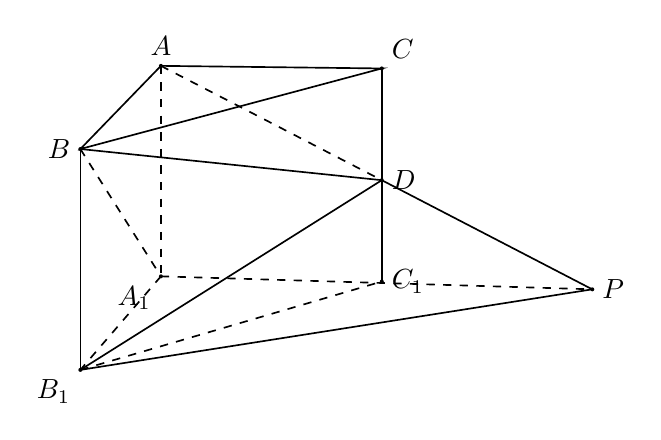
\begin{tikzpicture}[scale=0.66, >=stealth, semithick]
  \coordinate (A)  at (3.10,6.60);
  \coordinate (B)  at (1.55,5.00);
  \coordinate (C)  at (7.35,6.55);
  \coordinate (A1) at (3.10,2.55);
  \coordinate (B1) at (1.55,0.75);
  \coordinate (C1) at (7.35,2.45);
  \coordinate (D)  at (7.35,4.40);
  \coordinate (P)  at (11.40,2.30);

  % 可见棱（实线）
  \draw (A) -- (B) -- (C) -- cycle;
  \draw (B) -- (B1);
  \draw (C) -- (C1);
  \draw (B) -- (D);
  \draw (B1) -- (D);
  \draw (B1) -- (P);
  \draw (D) -- (P);

  % 被遮挡的棱（虚线）
  \draw[dashed] (A) -- (A1);
  \draw[dashed] (A1) -- (B1);
  \draw[dashed] (A1) -- (P);
  \draw[dashed] (B1) -- (C1);
  \draw[dashed] (B) -- (A1);
  \draw[dashed] (A) -- (D);

  \fill (A) circle (1.1pt);
  \fill (B) circle (1.1pt);
  \fill (C) circle (1.1pt);
  \fill (A1) circle (1.1pt);
  \fill (B1) circle (1.1pt);
  \fill (C1) circle (1.1pt);
  \fill (D) circle (1.1pt);
  \fill (P) circle (1.1pt);

  \node at (A)  [above] {$A$};
  \node at (B)  [left] {$B$};
  \node at (C)  [above right] {$C$};
  \node at (A1) [below left] {$A_1$};
  \node at (B1) [below left] {$B_1$};
  \node at (C1) [right] {$C_1$};
  \node at (D)  [right] {$D$};
  \node at (P)  [right] {$P$};
\end{tikzpicture}
\end{center}
\nopagebreak[4]
\Needspace{4\baselineskip}
\textbf{解析}

\Needspace{5\baselineskip}
以 $A$ 为原点，$\overrightarrow{AB}$，$\overrightarrow{AC}$，$\overrightarrow{AA_1}$ 为 $x$，$y$，$z$ 轴正方向建系（$AB=AC=AA_1=1$，$\angle BAC=90^\circ$，三棱柱为直棱柱，三轴两两垂直），则
\nopagebreak[4]
\[A(0,0,0),\ B(1,0,0),\ C(0,1,0),\ A_1(0,0,1),\ B_1(1,0,1),\ C_1(0,1,1).\]
$D$ 在棱 $CC_1$ 上，设 $D(0,1,t)$，$0<t\leqslant1$（$t=0$ 时 $D=C$，$AD$ 即 $AC$，与 $A_1C_1$ 平行无交点，不合题意）。

\gksubpart{(1)}
\Needspace{5\baselineskip}
直线 $AD$ 上的点为 $\lambda(0,1,t)$；直线 $A_1C_1$ 为 $\{(0,s,1)\}$。相交要求 $\lambda t=1$，故
\nopagebreak[4]
\[P\left(0,\frac1t,1\right),\qquad \overrightarrow{PB_1}=\left(1,-\frac1t,0\right).\]
\Needspace{5\baselineskip}
平面 $BDA_1$ 的法向量
\nopagebreak[4]
\[\boldsymbol n=\overrightarrow{BA_1}\times\overrightarrow{BD}=(-1,0,1)\times(-1,1,t)=(-1,\,t-1,\,-1).\]
\Needspace{5\baselineskip}
由 $PB_1\parallel$ 平面 $BDA_1$ 得 $\boldsymbol n\perp\overrightarrow{PB_1}$：
\nopagebreak[4]
\[\boldsymbol n\cdot\overrightarrow{PB_1}=-1+(t-1)\left(-\frac1t\right)+0=-1-1+\frac1t=\frac1t-2=0,\]
故 $t=\dfrac12$，即 $D$ 为 $CC_1$ 的中点，$CD=C_1D=\dfrac12$。

\gksubpart{(2)}
$D\left(0,1,\dfrac12\right)$。平面 $AA_1D$ 过 $A$，$A_1$，$D$，三点 $x$ 坐标均为 $0$，即平面 $x=0$，取 $\boldsymbol n_1=(1,0,0)$。平面 $BA_1D$ 取 $\boldsymbol n_2=(2,1,2)$，验证 $\boldsymbol n_2\cdot\overrightarrow{BA_1}=-2+0+2=0$，$\boldsymbol n_2\cdot\overrightarrow{BD}=-2+1+1=0$，故 $\boldsymbol n_2$ 为其法向量。

\Needspace{5\baselineskip}
为了定出二面角的平面角（而非两法向量的夹角），在棱 $A_1D$ 上取垂直于棱、分别指向 $A$ 与 $B$ 的向量：
\nopagebreak[4]
\[\boldsymbol u=(0,-1,-2),\qquad \boldsymbol v=(5,-2,-4).\]
\Needspace{5\baselineskip}
检验：$\overrightarrow{A_1D}=\left(0,1,-\dfrac12\right)$，$\boldsymbol u\cdot\overrightarrow{A_1D}=-1+1=0$，$\boldsymbol v\cdot\overrightarrow{A_1D}=-2+2=0$；$\overrightarrow{A_1A}=(0,0,-1)$，$\boldsymbol u\cdot\overrightarrow{A_1A}=2>0$；$\overrightarrow{A_1B}=(1,0,-1)$，$\boldsymbol v\cdot\overrightarrow{A_1B}=5+4=9>0$。故二面角的平面角余弦为
\nopagebreak[4]
\[\cos\theta=\frac{\boldsymbol u\cdot\boldsymbol v}{|\boldsymbol u||\boldsymbol v|}=\frac{0+2+8}{\sqrt5\cdot3\sqrt5}=\frac{10}{15}=\frac23.\]
与 $|\cos\langle\boldsymbol n_1,\boldsymbol n_2\rangle|=\dfrac{2}{1\cdot3}=\dfrac23$ 一致，且由上述同侧检验知平面角为锐角，余弦为正。

\gksubpart{(3)}
\Needspace{5\baselineskip}
$B_1(1,0,1)$，$D\left(0,1,\dfrac12\right)$，$P(0,2,1)$。于是
\nopagebreak[4]
\[\overrightarrow{B_1D}=\left(-1,1,-\frac12\right),\qquad \overrightarrow{B_1P}=(-1,2,0),\]
\Needspace{5\baselineskip}
法向量
\nopagebreak[4]
\[\overrightarrow{B_1D}\times\overrightarrow{B_1P}=\left(1,\frac12,-1\right),\]
\Needspace{5\baselineskip}
取 $\boldsymbol m=(2,1,-2)$。又 $\overrightarrow{B_1C}=(-1,1,-1)$，故点 $C$ 到平面 $B_1DP$ 的距离
\nopagebreak[4]
\[d=\frac{|\boldsymbol m\cdot\overrightarrow{B_1C}|}{|\boldsymbol m|}=\frac{|{-2+1+2}|}{3}=\frac13.\]

二次复算（平面方程法）：由 $B_1(1,0,1)$，$D\left(0,1,\dfrac12\right)$，$P(0,2,1)$ 可直接写出平面 $B_1DP$ 的方程 $2x+y-2z=0$（三点均满足），点 $C(0,1,0)$ 到它的距离为 $\dfrac{|2\cdot0+1-2\cdot0|}{\sqrt{4+1+4}}=\dfrac13$，与坐标法一致。

\gkanswer{答案（1）：证明见解析（$CD=C_1D=\dfrac12$）}

\gkanswer{答案（2）：$\dfrac23$}

\gkanswer{答案（3）：$\dfrac13$。}

\end{answer}
\begin{answer}
\gksolhead{20}{}

\textbf{题目}：

\Needspace{5\baselineskip}
设 $d$ 为非零实数，
\nopagebreak[4]
\[a_n=\frac1n\left[\mathrm C_n^1d+2\mathrm C_n^2d^2+\cdots+(n-1)\mathrm C_n^{n-1}d^{n-1}+n\mathrm C_n^nd^n\right]\quad(n\in\mathbf N^*).\]

（1） 写出 $a_1$，$a_2$，$a_3$ 并判断 $\{a_n\}$ 是否为等比数列。若是，给出证明；若不是，说明理由；

（2） 设 $b_n=nda_n$（$n\in\mathbf N^*$），求数列 $\{b_n\}$ 的前 $n$ 项和 $S_n$。

\Needspace{4\baselineskip}
\textbf{解析}

\Needspace{5\baselineskip}
记 $T_n=\displaystyle\sum_{k=1}^{n}k\mathrm C_n^kd^k$。由 $(1+d)^n=\sum\limits_{k=0}^{n}\mathrm C_n^kd^k$ 两边对 $d$ 求导得
\nopagebreak[4]
\[\sum_{k=1}^{n}k\mathrm C_n^kd^{k-1}=n(1+d)^{n-1},\]
\Needspace{5\baselineskip}
两边乘 $d$：
\nopagebreak[4]
\[T_n=nd(1+d)^{n-1}.\]
\Needspace{5\baselineskip}
故
\nopagebreak[4]
\[a_n=\frac{T_n}{n}=d(1+d)^{n-1}.\]

\gksubpart{(1)}
\Needspace{5\baselineskip}
依次得
\nopagebreak[4]
\[a_1=d,\qquad a_2=d(1+d),\qquad a_3=d(1+d)^2.\]
因 $d\neq0$，$a_1\neq0$。

若 $d=-1$，则 $a_1=-1$，$a_2=a_3=\cdots=0$。此时 $a_2=0$ 而 $a_1\neq0$，$\dfrac{a_2}{a_1}=0$ 但 $\dfrac{a_3}{a_2}$ 无意义，故 $\{a_n\}$ \textbf{不是}等比数列。

\Needspace{5\baselineskip}
若 $d\neq-1$，则 $1+d\neq0$，$a_n=d(1+d)^{n-1}\neq0$，且
\nopagebreak[4]
\[\frac{a_{n+1}}{a_n}=\frac{d(1+d)^{n}}{d(1+d)^{n-1}}=1+d\]
为与 $n$ 无关的常数，故 $\{a_n\}$ 是首项 $d$、公比 $1+d$ 的等比数列。

\gksubpart{(2)}
\Needspace{5\baselineskip}
由（1）得
\nopagebreak[4]
\[b_n=nda_n=nd^2(1+d)^{n-1}.\]
\Needspace{5\baselineskip}
记 $q=1+d$。因 $d\neq0$，故 $q\neq1$，可错位相减：
\nopagebreak[4]
\[S_n=d^2\sum_{k=1}^{n}kq^{k-1},\qquad qS_n=d^2\sum_{k=1}^{n}kq^{k},\]
\nopagebreak[4]
\[(1-q)S_n=d^2\left[\sum_{k=1}^{n}kq^{k-1}-\sum_{k=1}^{n}kq^{k}\right]=d^2\left[\sum_{j=0}^{n-1}q^{j}-nq^{n}\right]=d^2\left[\frac{1-q^{n}}{1-q}-nq^{n}\right].\]
\Needspace{5\baselineskip}
又 $1-q=-d$，故 $\dfrac{d^2}{(1-q)^2}=1$，上式两边除以 $1-q$：
\nopagebreak[4]
\[S_n=\frac{d^2}{(1-q)^2}(1-q^{n})-\frac{nd^2q^{n}}{1-q}=(1-q^{n})+nd\,q^{n}.\]
\Needspace{5\baselineskip}
回代 $q=1+d$：
\nopagebreak[4]
\[S_n=1+q^n(nd-1)=1+(nd-1)(1+d)^n.\]

二次复算：$n=1$ 时 $S_1=1+(d-1)(1+d)=1+d^2-1=d^2=b_1$；$n=2$ 时 $S_2=1+(2d-1)(1+d)^2$，而 $b_1+b_2=d^2+2d^2(1+d)=d^2(3+2d)$，两者相等（展开 $(2d-1)(1+2d+d^2)=2d+4d^2+2d^3-1-2d-d^2=3d^2+2d^3-1$，加 $1$ 即 $d^2(3+2d)$），一致。

\gkanswer{答案（1）：$a_1=d$，$a_2=d(1+d)$，$a_3=d(1+d)^2$；$d=-1$ 时不是等比数列，$d\neq-1$ 时为等比数列，公比 $1+d$}

\gkanswer{答案（2）：$S_n=1+(nd-1)(1+d)^n$。}

\end{answer}
\begin{answer}
\gksolhead{21}{}

\textbf{题目}：

椭圆有两顶点 $A(-1,0)$，$B(1,0)$，过其焦点 $F(0,1)$ 的直线 $l$ 与椭圆交于 $C$，$D$ 两点，并与 $x$ 轴交于点 $P$。直线 $AC$ 与直线 $BD$ 交于点 $Q$。

（1） 当 $|CD|=\dfrac32\sqrt2$ 时，求直线 $l$ 的方程；

（2） 当点 $P$ 异于 $A$，$B$ 两点时，求证：$\overrightarrow{OP}\cdot\overrightarrow{OQ}$ 为定值。
\nopagebreak[4]
\begin{center}% 2011 年四川卷理科第 21 题：椭圆 x^2+y^2/2=1，顶点 A(-1,0)、B(1,0)，焦点 F(0,1)，
%   过 F 的直线 l 交椭圆于 C、D，交 x 轴于 P，直线 AC 与 BD 交于 Q。
% 来源 PDF：普通高考/2011/2011四川理.pdf，SHA-256 116ce515679869425079ef4777505df3735ba4cba64847c9069b7d7acdb4fda4。
% 原页：第 2 页（A3 三栏）第 2 栏中部，书页码 702。
% 重绘依据：照原页——椭圆竖长（半轴 1 与 √2），A 为左顶点、B 为右顶点，F 在 O 上方；
%   l 自左上（过 D）经 F、C 交 x 轴于 B 右侧的 P，并越过 P 继续向右下；
%   AC 自 A 过 C 向右上延长，BD 自 B 过 D 向左上延长，二者交于 Q（椭圆内、O 右侧）。
%   取 l 的斜率 k=-0.55，各点按解析式算得，不按原页比例。
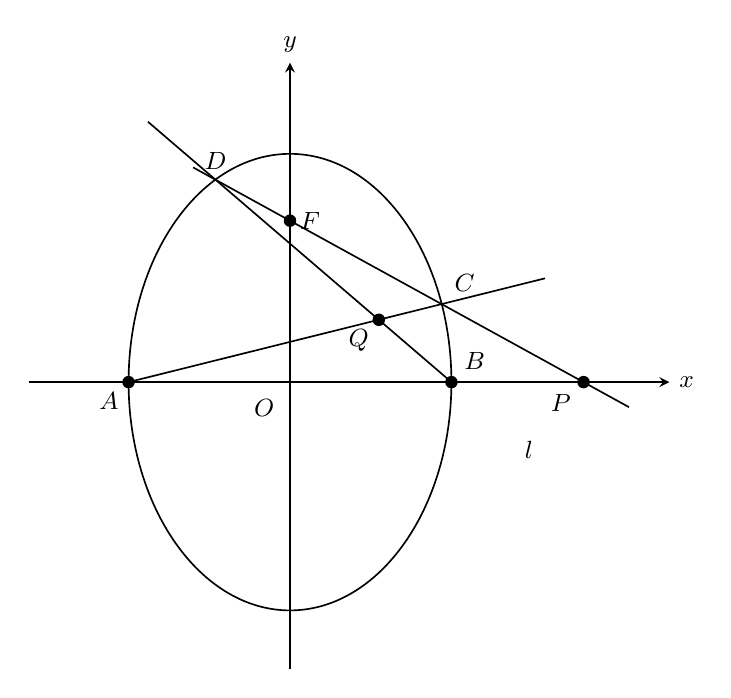
\begin{tikzpicture}[scale=2.05, >=stealth, semithick, font=\small]
  % 坐标轴
  \draw[->] (-1.62,0) -- (2.35,0) node[right] {$x$};
  \draw[->] (0,-1.78) -- (0,1.98) node[above] {$y$};

  % 椭圆
  \draw (0,0) ellipse (1 and 1.41421);

  % 各点
  \coordinate (A) at (-1,0);
  \coordinate (B) at (1,0);
  \coordinate (F) at (0,1);
  \coordinate (C) at (0.9397,0.4832);
  \coordinate (D) at (-0.4619,1.2540);
  \coordinate (P) at (1.8182,0);
  \coordinate (Q) at (0.55,0.3861);

  % 直线 l
  \draw (-0.60,1.330) -- (2.10,-0.155);
  % 直线 AC、BD 及其延长
  \draw (A) -- (1.58,0.643);
  \draw (B) -- (-0.88,1.613);

  \fill (A) circle (1.1pt);
  \fill (B) circle (1.1pt);
  \fill (F) circle (1.1pt);
  \fill (P) circle (1.1pt);
  \fill (Q) circle (1.1pt);

  \node at (A) [below left] {$A$};
  \node at (B) [above right=1pt] {$B$};
  \node at (F) [right] {$F$};
  \node at (C) [above right=1pt] {$C$};
  \node at (D) [above] {$D$};
  \node at (P) [below left=1pt] {$P$};
  \node at (Q) [below left] {$Q$};
  \node at (-0.16,-0.16) {$O$};
  \node at (1.48,-0.42) {$l$};
\end{tikzpicture}
\end{center}
\nopagebreak[4]
\Needspace{4\baselineskip}
\textbf{解析}

\Needspace{5\baselineskip}
由顶点 $A(-1,0)$，$B(1,0)$ 知短半轴 $b=1$；焦点 $F(0,1)$ 在 $y$ 轴上，故长轴在 $y$ 轴上，$c=1$，$a^2=b^2+c^2=2$，椭圆为
\nopagebreak[4]
\[x^2+\frac{y^2}{2}=1\iff 2x^2+y^2=2.\]

\gksubpart{(1)}
\Needspace{5\baselineskip}
设 $l\colon y=kx+1$（$l$ 与 $x$ 轴有交点，故 $k\neq0$；竖直情形单独讨论）。代入椭圆方程：
\nopagebreak[4]
\[2x^2+(kx+1)^2=2\iff(k^2+2)x^2+2kx-1=0.\]
\Needspace{5\baselineskip}
设 $C(x_1,y_1)$，$D(x_2,y_2)$，则
\nopagebreak[4]
\[x_1+x_2=-\frac{2k}{k^2+2},\qquad x_1x_2=-\frac{1}{k^2+2},\]
\nopagebreak[4]
\[|x_1-x_2|=\sqrt{(x_1+x_2)^2-4x_1x_2}=\frac{\sqrt{4k^2+4(k^2+2)}}{k^2+2}=\frac{2\sqrt2\sqrt{1+k^2}}{k^2+2}.\]
\Needspace{5\baselineskip}
故弦长
\nopagebreak[4]
\[|CD|=\sqrt{1+k^2}\,|x_1-x_2|=\frac{2\sqrt2(1+k^2)}{k^2+2}.\]
\Needspace{5\baselineskip}
由 $|CD|=\dfrac32\sqrt2$ 得
\nopagebreak[4]
\[\frac{2(1+k^2)}{k^2+2}=\frac32\iff4+4k^2=6+3k^2\iff k^2=2,\]
即 $k=\pm\sqrt2$。此时 $l\colon y=\sqrt2x+1$ 或 $y=-\sqrt2x+1$。

另需排除竖直线 $x=0$：它与椭圆交于 $(0,\pm\sqrt2)$，$|CD|=2\sqrt2\neq\dfrac32\sqrt2$，不合。

\gksubpart{(2)}
由 $l$ 与 $x$ 轴交于 $P$ 知 $k\neq0$；由附加条件 $P\neq A$，$B$ 知 $k\neq\pm1$（$k=1$ 时 $P=A$，$k=-1$ 时 $P=B$，此时 $C$ 或 $D$ 与 $A$ 或 $B$ 重合）。设 $l\colon y=kx+1$（$k\neq0$），$l\perp x$ 轴的情形见本节末的补充说明。

\Needspace{5\baselineskip}
令 $y=0$ 得 $P\left(-\dfrac1k,0\right)$。设 $Q(x_Q,y_Q)$。$Q$ 在直线 $AC$ 上，也在直线 $BD$ 上：
\nopagebreak[4]
\[\frac{y_Q}{x_Q+1}=\frac{y_1}{x_1+1},\qquad \frac{y_Q}{x_Q-1}=\frac{y_2}{x_2-1}.\]
\Needspace{5\baselineskip}
两式相除消去 $y_Q$：
\nopagebreak[4]
\[\frac{x_Q-1}{x_Q+1}=\frac{y_1(x_2-1)}{y_2(x_1+1)}.\]
\Needspace{5\baselineskip}
记 $A_1=(kx_1+1)(x_2-1)$，$A_2=(kx_2+1)(x_1+1)$（用了 $y_i=kx_i+1$），则 $A_1(x_Q+1)=A_2(x_Q-1)$，即
\nopagebreak[4]
\[x_Q=\frac{A_1+A_2}{A_2-A_1}.\]
\Needspace{5\baselineskip}
展开 $A_1+A_2=2kx_1x_2+(x_1+x_2)+k(x_2-x_1)$，$A_2-A_1=k(x_1+x_2)+(x_1-x_2)+2$。代入韦达定理及 $x_1-x_2=\dfrac{2\sqrt2\sqrt{1+k^2}}{k^2+2}$：
\nopagebreak[4]
\[A_1+A_2=\frac{-2k-2k-2\sqrt2k\sqrt{1+k^2}}{k^2+2}=\frac{-2k\left(2+\sqrt2\sqrt{1+k^2}\right)}{k^2+2},\]
\nopagebreak[4]
\[A_2-A_1=\frac{-2k^2+2\sqrt2\sqrt{1+k^2}+2(k^2+2)}{k^2+2}=\frac{2\left(2+\sqrt2\sqrt{1+k^2}\right)}{k^2+2}.\]
\Needspace{5\baselineskip}
两式中含 $\sqrt{1+k^2}$ 的括号相同且为正，约去得
\nopagebreak[4]
\[x_Q=-k.\]
\Needspace{5\baselineskip}
于是
\nopagebreak[4]
\[\overrightarrow{OP}\cdot\overrightarrow{OQ}=\left(-\frac1k\right)(-k)+0\cdot y_Q=1,\]
为定值 $1$。

补充说明：当 $l\perp x$ 轴（$l\colon x=0$）时，$C(0,\sqrt2)$，$D(0,-\sqrt2)$，$k_{AC}=\sqrt2=k_{BD}$，两直线平行，题设中的点 $Q$ 不存在；题面只排除了 $P$ 与 $A$，$B$ 重合，未排除此情形，故第（2）问按 $l$ 斜率存在且 $k\neq0$ 理解。

\Needspace{5\baselineskip}
二次复算：取 $k=-2$，得
\nopagebreak[4]
\[
\begin{aligned}
C&\left(\frac{2+\sqrt{10}}{6},\,1-2\cdot\frac{2+\sqrt{10}}{6}\right),\\
D&\left(\frac{2-\sqrt{10}}{6},\,1-2\cdot\frac{2-\sqrt{10}}{6}\right),
\end{aligned}
\]
数值上 $C\approx(0.860,-0.721)$，$D\approx(-0.194,1.388)$，$P=(0.5,0)$，$Q=(2,-1.163)$，$\overrightarrow{OP}\cdot\overrightarrow{OQ}=0.5\times2+0=1$，与结论吻合。

\gkanswer{答案（1）：$y=\sqrt2x+1$ 或 $y=-\sqrt2x+1$}

\gkanswer{答案（2）：定值为 $1$。}

\end{answer}
\begin{answer}
\gksolhead{22}{}

\textbf{题目}：

已知函数 $f(x)=\dfrac23x+\dfrac12$，$h(x)=\sqrt x$。

（1） 设函数 $F(x)=f(x)-h(x)$，求 $F(x)$ 的单调区间与极值；

\Needspace{5\baselineskip}
（2） 设 $a\in\mathbf R$，解关于 $x$ 的方程
\nopagebreak[4]
\[\log_4\left[\frac32f(x-1)-\frac34\right]=\log_2h(a-x)-\log_2h(4-x);\]

（3） 试比较 $f(100)h(100)-\displaystyle\sum_{k=1}^{100}h(k)$ 与 $\dfrac16$ 的大小。

\Needspace{4\baselineskip}
\textbf{解析}

\gksubpart{(1)}
\Needspace{5\baselineskip}
$F(x)=\dfrac23x+\dfrac12-\sqrt x$，定义域 $[0,+\infty)$，
\nopagebreak[4]
\[F'(x)=\frac23-\frac{1}{2\sqrt x}=\frac{4\sqrt x-3}{6\sqrt x}.\]
\Needspace{5\baselineskip}
由 $F'(x)=0$ 得 $\sqrt x=\dfrac34$，$x=\dfrac9{16}$。当 $0<x<\dfrac9{16}$ 时 $4\sqrt x<3$，$F'<0$；当 $x>\dfrac9{16}$ 时 $F'>0$。故 $F$ 在 $\left(0,\dfrac9{16}\right)$ 上单调递减，在 $\left(\dfrac9{16},+\infty\right)$ 上单调递增，
\nopagebreak[4]
\[F\left(\frac9{16}\right)=\frac23\cdot\frac9{16}+\frac12-\frac34=\frac38+\frac12-\frac34=\frac18,\]
为极小值（也是最小值），无极大值。

\gksubpart{(2)}
\Needspace{5\baselineskip}
先化简被开方式：
\nopagebreak[4]
\[\frac32f(x-1)-\frac34=\frac32\left[\frac23(x-1)+\frac12\right]-\frac34=(x-1)+\frac34-\frac34=x-1.\]
\Needspace{5\baselineskip}
方程化为
\nopagebreak[4]
\[\log_4(x-1)=\log_2h(a-x)-\log_2h(4-x)=\frac12\log_2(a-x)-\frac12\log_2(4-x),\]
\Needspace{5\baselineskip}
即
\nopagebreak[4]
\[\frac12\log_2(x-1)=\frac12\log_2\frac{a-x}{4-x}\iff x-1=\frac{a-x}{4-x}.\]
\Needspace{5\baselineskip}
定义域要求 $\log_4(x-1)$ 有意义、$\log_2h(a-x)$ 与 $\log_2h(4-x)$ 有意义，即
\nopagebreak[4]
\[x>1,\qquad x<4,\qquad a>x.\]
\Needspace{5\baselineskip}
在此前提下，$x-1=\dfrac{a-x}{4-x}$ 两边乘 $4-x>0$：
\nopagebreak[4]
\[(x-1)(4-x)=a-x\iff -x^2+5x-4=a-x\iff x^2-6x+4+a=0,\]
\Needspace{5\baselineskip}
故
\nopagebreak[4]
\[x=3\pm\sqrt{5-a}\quad(a\leqslant5).\]
记 $t=\sqrt{5-a}\geqslant0$，则 $a=5-t^2$，两根为 $x=3+t$ 与 $x=3-t$。逐一检验三个条件：

\begin{itemize}
\item 对 $x=3+t$：$x<4\iff t<1$；$a>x\iff 5-t^2>3+t\iff t^2+t-2<0\iff t<1$。故 $0\leqslant t<1$ 时可用。
\item 对 $x=3-t$：$x>1\iff t<2$；$a>x\iff 5-t^2>3-t\iff t^2-t-2<0\iff t<2$。故 $0\leqslant t<2$ 时可用。
\end{itemize}

所以 $t\in[0,1)$ 时两根都在定义域内；$t\in[1,2)$ 时只剩 $x=3-t$；$t\geqslant2$ 时无解。注意 $t=0$ 时两根重合于 $x=3$。换算回 $a$（$a=5-t^2$，$t$ 随 $a$ 减小而增大）：

\begin{itemize}
\item $a\leqslant1$（$t\geqslant2$）：无解；
\item $1<a\leqslant4$（$1\leqslant t<2$）：唯一解 $x=3-\sqrt{5-a}$；
\item $4<a<5$（$0<t<1$）：两解 $x=3\pm\sqrt{5-a}$；
\item $a=5$（$t=0$）：唯一解 $x=3$；
\item $a>5$：无解（$5-a<0$）。
\end{itemize}

\Needspace{5\baselineskip}
代回检验：$a=4$（$t=1$）时两根为 $2$ 与 $4$，其中 $x=4$ 使 $4-x=0$，舍去；$x=2$ 时左边 $\log_4(1)=0$，右边 $\log_2\sqrt2-\log_2\sqrt2=0$，成立。$a=\dfrac92$（$t=\dfrac{\sqrt2}{2}$）时取 $x=3+\dfrac{\sqrt2}{2}$，则 $x-1=\dfrac{4+\sqrt2}{2}$，而
\nopagebreak[4]
\[\frac{a-x}{4-x}=\frac{\frac32-\frac{\sqrt2}{2}}{1-\frac{\sqrt2}{2}}=\frac{3-\sqrt2}{2-\sqrt2}=\frac{(3-\sqrt2)(2+\sqrt2)}{2}=\frac{4+\sqrt2}{2},\]
两边相等；另一根 $x=3-\dfrac{\sqrt2}{2}$ 同理（$x-1=\dfrac{4-\sqrt2}{2}$，$\dfrac{a-x}{4-x}=\dfrac{3+\sqrt2}{2+\sqrt2}=\dfrac{4-\sqrt2}{2}$）。

\gksubpart{(3)}
\Needspace{5\baselineskip}
先算首项：
\nopagebreak[4]
\[f(100)h(100)=\left(\frac23\cdot100+\frac12\right)\sqrt{100}=\left(\frac{200}{3}+\frac12\right)\cdot10=\frac{403}{6}\cdot10=\frac{2015}{3}.\]
\Needspace{5\baselineskip}
对 $k=2,3,\cdots,100$，函数 $\sqrt t$ 在 $[k-1,k]$ 上连续且严格凹（$\sqrt t$ 的二阶导数为 $-\dfrac{1}{4}t^{-3/2}<0$），由凹函数的梯形估计（弦在曲线下方）：
\nopagebreak[4]
\[\frac{\sqrt{k-1}+\sqrt{k}}{2}<\int_{k-1}^{k}\sqrt t\,\mathrm dt=\frac23\left[k^{\frac32}-(k-1)^{\frac32}\right],\]
\Needspace{5\baselineskip}
即
\nopagebreak[4]
\[\sqrt{k-1}+\sqrt{k}<\frac43\left[k^{\frac32}-(k-1)^{\frac32}\right].\]
\Needspace{5\baselineskip}
对 $k=2,\cdots,100$ 求和，左端
\nopagebreak[4]
\[\sum_{k=2}^{100}\left(\sqrt{k-1}+\sqrt{k}\right)=2\sum_{k=1}^{100}\sqrt k-\sqrt1-\sqrt{100}=2\sum_{k=1}^{100}\sqrt k-11,\]
\Needspace{5\baselineskip}
右端为裂项和
\nopagebreak[4]
\[\frac43\sum_{k=2}^{100}\left[k^{\frac32}-(k-1)^{\frac32}\right]=\frac43\left(100^{\frac32}-1\right)=\frac43(1000-1)=1332.\]
\Needspace{5\baselineskip}
故
\nopagebreak[4]
\[2\sum_{k=1}^{100}\sqrt k-11<1332\implies\sum_{k=1}^{100}\sqrt k<\frac{1343}{2}.\]
\Needspace{5\baselineskip}
于是
\nopagebreak[4]
\[f(100)h(100)-\sum_{k=1}^{100}h(k)>\frac{2015}{3}-\frac{1343}{2}=\frac{4030-4029}{6}=\frac16.\]
即前者大于 $\dfrac16$。

二次复算（数值）：直接求和得 $\displaystyle\sum_{k=1}^{100}\sqrt k\approx671.462$，而 $\dfrac{2015}{3}\approx671.667$，差约 $0.204>\dfrac16\approx0.167$，与证明一致；上式给出的上界 $\dfrac{1343}{2}=671.5$ 也确实小于 $\dfrac{2015}{3}$。

\gkanswer{答案（1）：减区间 $\left(0,\dfrac{9}{16}\right)$，增区间 $\left(\dfrac{9}{16},+\infty\right)$，极小值 $\dfrac18$，无极大值}

\gkanswer{答案（2）：当 $a\leqslant1$ 时无解；当 $1<a\leqslant4$ 时 $x=3-\sqrt{5-a}$；当 $4<a<5$ 时 $x=3\pm\sqrt{5-a}$；当 $a=5$ 时 $x=3$；当 $a>5$ 时无解}

\gkanswer{答案（3）：大于 $\dfrac16$。}

\end{answer}